\section{Irregularity Parameter estimation}
\label{sec:irregularity_parameter_estimation}
The generation of realistic ionospheric scintillation effects with the approach described in section \ref{sec:ps_theory} depends entirely on the choice of the aforementioned irregularity parameters. In this view, recent studies have proposed different manners of estimating these parameters by matching a modeled intensity SDF with a real (measured) intensity SDF from a GNSS receiver. 

However, in the lack of real data to fully characterize the irregularity parameters for both weak, moderate and strong scintillation cases, researchers can also choose these parameters based on the comprehensive evaluation of the two-component power law spectred done in \cite{Carrano2016OverviewOfTwoComponentPowerLaw}.
\subsection{Brief Literature Review}

\textcite{CarranoBrazil2012} have initially proposed and evaluated a irregularity parameter estimation (IPE) technique based on a iterative algorithm for evaluating the turbulance strength parameter and the spectral index of a one-component power law model, as well as the zonal drift of the ionosphere. This algorithm relies on the minimization of a metric that measures similarity degree between a modeled and a realistic signal intensity SDF, obtained via detrended real data, by using a downhill simplex algorithm. 

This algorithm was also used in recent works that evaluates the quality of a two-component power-law model in representing the statistics of real ionospheric scintillation events for static \cite{JiaoMultifrequencyScintillationOnGPSSignalsStaticPlatforms2018} and dynamic platforms \cite{JiaoScintillationOnGPSSignalsForDynamicPlatforms2018}. In addition, the work \cite{xuTwoparameterMultifrequencyGPS2020} was also developed using the iterative IPE.

It is important to mention that \textcite{carrano2017maximum} recently presented a more robust solution that is based on maximum likelihood estimation of the irregularity parameters, which was further used to characterize the intermadiate-scale ionospheric structure in \cite{Carrano2018IntermadiateScaleCharacterization}. The author justify that this approach is more robust on the argument that the previous one relies on the Gaussianity and uncorrelatedness of the residuals, while this novel one provides a more comprehensive solution, since this assumption is no longer necessary.

Therefore, since only few algorithms irregularity parameter estimation algorithms were developed, and most of them only tries to find them by fitting a modeled intensity spectrum in a real received signal intensity spectrum, and completly neglects the phase spectrum in this task, there is a necessity of the development of more reliable and computationally efficient algorithms that don't make restricting prior assumptions, such as linearity of the variables.

In order to facilitate the usage of the TPPSM for researchers that are not familiar with phase screen models, \cite{xuTwoparameterMultifrequencyGPS2020} proposed the usage of mapping functions that relates the universal turbulance strength $U$ and the time scaling parameter $\rho_F / v_{eff}$ to the widely used scintillation indices $S_4$ and the $\tau_0$, which are related to the scintillation severity and the decorrelation time, respectively. This work analyzed a large data set of recorded GNSS signals during scintillation events that happened at Ascension Island and Hong Kong.

Despite the usefulness of this approach for simulating moderate and severe ionospheric scintillation events, it is not well-suited for simulating low-intensity ionospheric scintillation events, since the proposed mapping methodology only comprehends $S_4$ values that ranges from 0.5883 to 1.001 \cite[\textit{Libraries/Utilities/ParaMapping.m}]{githubGitHubCusenselabgnssscintillationsimulator_2param}. After testing the model for mild scintillation cases of $S_4$ ($S_4 < 0.3$), negative values of the universal strength parameter $U$ were obatined, which might lead to unrealistic ionospheric scintillation scenarios. An example is shown in figure \ref{fig:low_scintillation_test}.

Therefore, if one wants to use the TPPSM framework to simulate scintillation for any level severity, it is mandatory to apply the direct values of the irregularity parameters by either using a prior study at hand, or obtain them by processing real intensity data using an IPE algorithm.

\begin{figure}
    \centering
    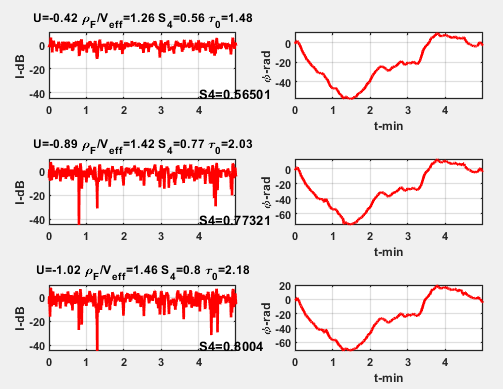
\includegraphics[width=0.40\textwidth]{figures/Low_intensity_test.png}
    \caption{Amplitude and phase scintillation time series obtained from the current version of the two-parameter scintillation model available at \url{https://github.com/cu-sense-lab/gnss-scintillation-simulator_2-param}, for a receiver positioned at Hong Kong (\texttt{userInput.RXPos = [0.3876 1.9942 59.6780]}), moving at 100 m/s at the eastward direction (\texttt{userInput.RXVel = [100 0 0]}), at 10:00:00 UTC in the date 2014/01/02, for the PRN number 18. The chosen values of $S_4$ and $\tau_0$ were 0.2 and 0.7, respectively.}
    \label{fig:low_scintillation_test}
\end{figure}

\subsection{Common Values for Irregularity Parameters for Weak and Strong Scattering}
\label{subsec:common_values_irr_param}
It is possible to observe from \cite[Section 4.4, Figures 7a, 7b, 8a, 8b]{Carrano2016OverviewOfTwoComponentPowerLaw} that, for the case of a one-component power law (named in this study as the \textit{unmodified power law}), the values of scintillation intensity index varies within the range $0.2 < S_4 < 0.4$ and the normalized intensity correlation length $\xi = \xi_c = r / \rho_F$, where $r=r_c$ is defined as the spatial separation for which the intensity correlation decreases to 50\%, varies from $0.2 < \xi_c < 2 s$ for the case when $U = 0.1$ for the values of spectral index within $1.5 < p < 4.5$. Therefore, we can consider $U < 0.1$ and $p=3$ as a feasible set of irregularity parameters for the weak scattering regime (note that there is no spectral break in the one-component power law model).

In addition, it is important to emphasize here that there is a high degree of similarity for the values of $S_4$ and $\xi_c$ in the limiting cases of the two-component power law depicted by \cite[Section 4.4, Figures 7c, 7d, 7e, 7f, 8c, 8d, 8e, 8f]{Carrano2016OverviewOfTwoComponentPowerLaw}, given that $U = U_1 = U_2 \ll 1$. Thus, it is justified the usage of a one-component power law model for this case.

Interestingly, in \cite[Section 4.1]{Carrano2016OverviewOfTwoComponentPowerLaw}, it is noted that the case when $p = 3$ characterizes the least intensity spectral widening and the longest correlation length scenario.

According to \cite{xuTwoparameterMultifrequencyGPS2020}, after using the iterative IPE, it was found that the mean values for $\left\{ \mu_0, p_1, p_2 \right\}$ for the strong scattering regime were 0.55, 2.45 and 3.7, respectively. It is possible to observe the distribution of the estimated parameters at the figure 5 of this same study. In this case, according to \cite[section 3.2.3]{Carrano2016OverviewOfTwoComponentPowerLaw}, this characterizes it as "Mixed-Slope" spectra, where both outer and inner scale structures contribute mutually with distortions to the transmitted signal. Furthermore, it is possible to observe in \cite[Figure 6]{xuTwoparameterMultifrequencyGPS2020} that a value of $U=2$ generates a intensity spectra whose $S_4$ is approximately 0.9, which can be characterized as a severe scintillation \cite[Section III, subsection A]{humphreysDatadrivenTestbedEvaluating2010}.

At the time of the development of this report, it was not possible to find relevant studies that tried to estimate the irrregularity parameters for GNSS signals under a moderate scattering regime. With that, we can reasonably assume that their values must lie within the range of the parameter set that defines the weak and strong scattering regimes.

In summary, we propose that the following irregularity parameter sets can be used as default for simulating weak, moderate and severe scattering regimes:
\begin{itemize}
    \item \textbf{Weak Scatter:} $\left\{ U = 0.05, p_1 = p_2 = p = 3  \right\}$
    \item \textbf{Moderate Scatter:} $\left\{ U = 0.4, \mu_0 = 0.7, p_1 = 2.7, p_2 = 3.3 \right\}$
    \item \textbf{Strong Scatter:} $\left\{ U = 2, \mu_0 = 0.55, p_1 = 2.45, p_2 = 3.7 \right\}$
\end{itemize}